\section{An "Explosive" Transition}
In this paper we are going to take a deeper look into a specific type of percolation called explosive percolation, where the underlying concept is that the onset of percolation is delayed until a certain point where it then occurs at an accelerated rate.
This occurs when the underlying evolution process works in such a way that the largest cluster size $|C|$ is controlled.
We can think of a graph where multiple clusters might evolve separately without merging.
Collectively they take up a large portion of the graph but there isn't a percolating cluster yet due to the lack of connections between the them.
If at some point these clusters do begin to connect then the graph transitions to the percolating state.
For certain evolution processes it has been heavily debated whether or not the phase transition is continuous or not, so the aim of the next section is to summarize what we know to this point regarding the nature of the transition for said processes.









\subsection{A Selective Process}
This all started in the year 2000 when Dimitris Achlioptas raised an interesting question about how a graph of $n$ nodes would evolve under certain conditions \cite{BF}.
First we suppose that at each step $t$ in the evolution process two edges $e_t$ and $e_t'$ are evaluated, but only one of them is selected to be added to the graph.
Which of the proposed edges is selected is based only on the information contained in $e_1, e_1', ... e_{t-1}, e_{t-1}'$.
Does there exist an algorithm for adding edges to the graph such that with high probability a giant component does not appear until $t/n > 0.5$?
This process of evaluating $m \ge 2$ edges at each step is now referred to as an $m$-edge Achlioptas process.
In the next few sections we will see how a small change to the way edges are added can have a big impact on the evolution of the system.










\subsection{The First Look}
In 2001 Tom Bohman and Alan Frieze were the first to design and analyze an Achlioptas process in their paper "Avoiding a Giant Component" \cite{BF}, where they set out to answer Achlioptas' question.
This paper laid out the framework for the Bohman-Frieze (BF) model of graph evolution and showed that there does exist a process in which the appearance of a giant cluster is delayed; so the answer to Achlioptas' question is yes!
This can be seen in Fig. \ref{fig:ER_BF_transition} where the order parameter for the BF model remains smaller than for the ER model, but a little after $r = 0.5$ it begins to rise at a faster rate than in the ER model, eventually overtaking the ER model.

\begin{figure}[H]
	\centering
	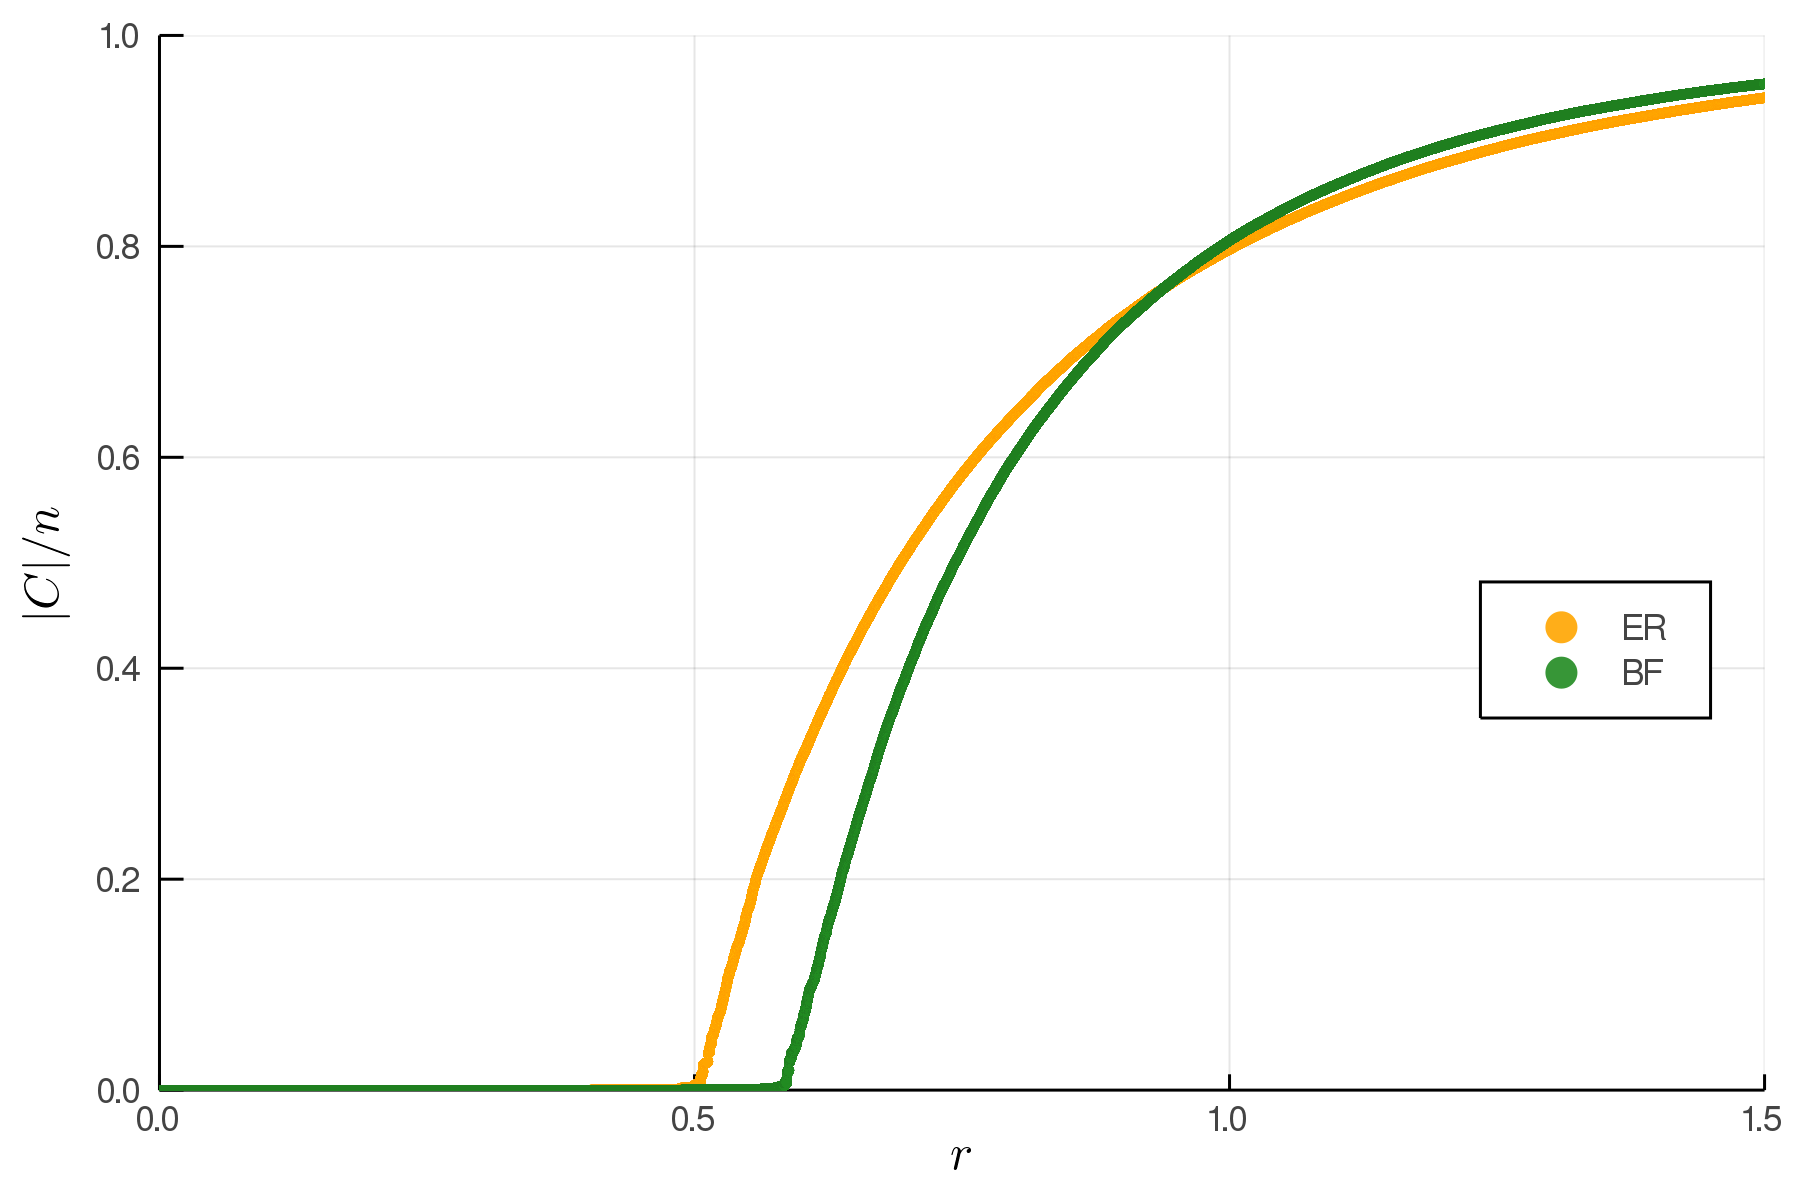
\includegraphics[width=350pt]{images/ER_BF_1e6_order_param.png}
	\caption{Bohman-Frieze Model Order Parameter, $n = 10^6$}
	\label{fig:ER_BF_transition}
\end{figure}

The algorithm they came up with randomly/uniformly samples and evaluates two edges $e_t$ and $e_t'$ at each step $t$, adding $e_t$ if it connects two isolated nodes and discarding $e_t'$, otherwise adding $e_t'$ and discarding $e_t$.
This is known as a bounded-size rule, which has since been generalized to a $K$ bounded-size rule where $e_t$ is added if it connects clusters of size smaller than $K$, otherwise $e_t'$ is added.
What this process does is equally discriminate against clusters of size greater than or equal to $K$.
It has been hypothesized that all bounded-size rules exhibit continuous phase transitions \cite{Spencer_Wormald}.

A form of the algorithm can be written in pseudocode as follows:
\begin{itemize}
	\item Let $T$ be the total number of edges to add to the graph.
	\item Let $A_t = \{e_1, e_2, ..., e_t\}$ be the set of accepted edges at step $t$.
	\item Let $e_t^1$ and $e_t^2$ be the two nodes which edge $e_t$ would connect.
	\item Let $C(e_t^i)$ be the cluster which $e_t^i$ belongs to.
\end{itemize}

\begin{algorithm}
	\caption{Bohman-Frieze}\label{Bohman-Frieze}
	\begin{algorithmic}[1]
		\Procedure{BF}{$T, K=2$}
		\State $A \gets \emptyset$
		\State $t \gets 1$
		\While{$t \le T$}
			\If{$|C(e_t^1)| < K$ and $|C(e_t^2)| < K$}
				\State $A \gets A \cup \{e_t\}$
			\Else
				\State $A \gets A \cup \{e_t'\}$
			\EndIf
			\State $t \gets t+1$
		\EndWhile
	\EndProcedure
	\end{algorithmic}
\end{algorithm}

A few years after their original paper, Bohman and Frieze published another paper with Nicholas Wormald titled "Avoidance of a giant component in half the edge set of a random graph" \cite{BFW}.
In this paper they designed a new algorithm (BFW) for adding edges to a graph that runs in phases beginning at $k = 2$.
Starting with $n$ isolated nodes, edges are randomly/uniformly sampled and evaluated one at a time.
If the edge being evaluated would create a cluster of size less than or equal to $k$ then the edge is accepted, otherwise the edge is rejected.
If edge is rejected and the ratio of accepted edges is less than the function $g(k) = 1/2 + \sqrt{1/(2k)}$, then the algorithm moves to the next phase.

A form of the algorithm can be written in pseudocode as follows:
\begin{itemize}
	\item Let $T$ be the total number of edges to add to the graph.
	\item Let $A_i = \{e_1, e_2, ..., e_i\}$ be the set of accepted edges at step $i$.
	\item Let $C(A)$ be the largest cluster in $A$.
\end{itemize}

\begin{algorithm}
	\caption{Bohman-Frieze-Wormald}\label{Bohman-Frieze-Wormald}
	\begin{algorithmic}[1]
		\Procedure{BFW}{$T$}
		\State $A \gets \emptyset$
		\State $k \gets 2$
		\State $t \gets 1$
		\State $i \gets 1$

		\While{$t \le T$}
			\If{$|C(A \cup \{e_i\})| \le k$}
				\State $A \gets A \cup \{e_i\}$
				\State $t \gets t+1$
				\State $i \gets i+1$
			\ElsIf{$|A|/i < g(k)$}
				\State $k \gets k+1$
			\Else
				\State $i \gets i+1$
			\EndIf
		\EndWhile
	\EndProcedure
	\end{algorithmic}
\end{algorithm}



\subsection{A Discontinuous Transition?}
The first mention of explosive percolation appeared in 2009 in the paper "Explosive Percolation in Random Networks" \cite{Achlioptas_1} by Dimitris Achlioptas, Raissa M. D’Souza, and Joel Spencer, which will henceforth be referred to as Achlioptas et al.
In this paper they laid out a method of choosing edges called the product rule (PR).
At each step $t$ in the evolution process two edges are selected randomly/uniformly and evaluated based on the product of the cluster sizes that the edges would connect.
More specifically, if edge $e_t$ connects clusters $C(e_t^1)$ and $C(e_t^2)$ and edge $e_t'$ connects clusters $C(e_t'^1)$ and $C(e_t'^2)$, then $e_t$ is accepted if $|C(e_t^1)| \cdot |C(e_t^2)| < |C(e_t'^1)| \cdot |C(e_t'^2)|$, otherwise $e_t'$ is accepted.

A form of the algorithm can be written in pseudocode as follows:
\begin{itemize}
	\item Let $T$ be the total number of edges to add to the graph.
	\item Let $A_t = \{e_1, e_2, ..., e_t\}$ be the set of accepted edges at step $t$.
	\item Let $e_t^1$ and $e_t^2$ be the two nodes which edge $e_t$ would connect.
	\item Let $C(e_t^i)$ be the cluster which $e_t^i$ belongs to.
\end{itemize}

\begin{algorithm}
	\caption{Product Rule}\label{Product-Rule}
	\begin{algorithmic}[1]
		\Procedure{PR}{$T$}
		\State $A \gets \emptyset$
		\State $t \gets 1$

		\While{$t \le T$}
			\If{$|C(e_t^1)| \cdot |C(e_t^2)| < |C(e_t'^1)| \cdot |C(e_t'^2)|$}
				\State $A \gets A \cup \{e_t\}$
				\State $t \gets t+1$
			\Else
				\State $A \gets A \cup \{e_t'\}$
				\State $t \gets t+1$
			\EndIf
		\EndWhile
	\EndProcedure
	\end{algorithmic}
\end{algorithm}

This is illustrated in Fig. \ref{fig:edge_selection} where the first proposed edge $e_t$ would connect the blue cluster of size 5 to the red cluster of size 3 and the second proposed edge $e_t'$ would connect the orange cluster of size 2 to the green cluster of size 4.
The product corresponding to $e_t$ is $5 \cdot 3 = 15$ whereas the product corresponding to $e_t$ is $2 \cdot 4 = 8$, so $e_t$ is rejected and $e_t'$ accepted.
If we were looking at Fig. \ref{fig:edge_selection} from within the framework of the BF model with $K = 1$, then $e_t$ would be rejected and $e_t$ accepted even though both the orange and green clusters are of size greater than $K$.

\begin{figure}[H]
	\centering
	\includegraphics[width=200pt, clip]{images/edge_selection.png}
	\caption{Edge Selection}
	\label{fig:edge_selection}
\end{figure}

Fig. \ref{fig:ER_BF_PR_transition} shows the order parameters for the ER, BF, and PR models, making it clear just how drastically different the PR model transition is than in the ER/BF models.
As can be seen the order parameter remains near zero for much longer until the critical point $r_c \approx 0.888...$ \cite{Achlioptas_1}, which is much later than the critical point in the ER model of $r_c = 0.5$.
Not long after the critical point is reached the order parameter appears to jump up discontinuously, which was a surprising find.

\begin{figure}[H]
	\centering
	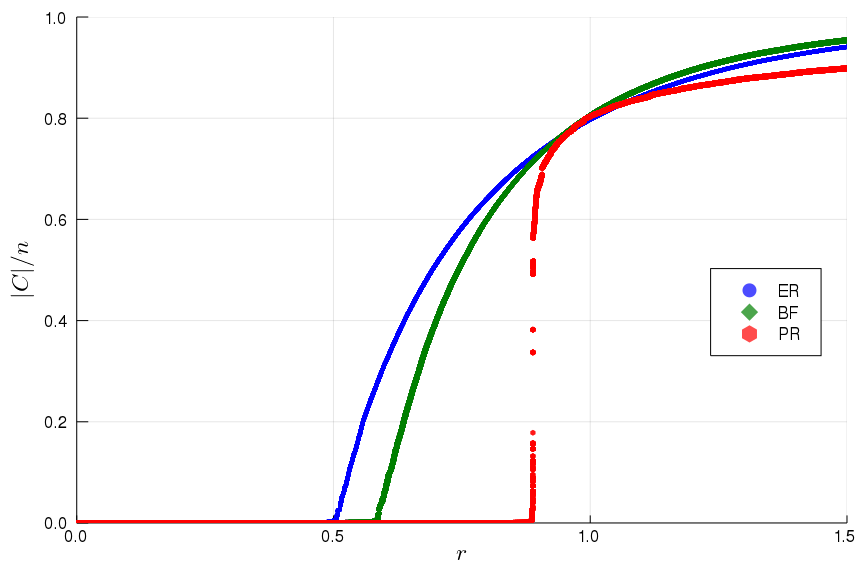
\includegraphics[width=350pt]{images/ER_BF_PR_1e6_order_param.png}
	\caption{Product Rule Model Order Parameter, $n = 10^6$}
	\label{fig:ER_BF_PR_transition}
\end{figure}

In their paper they analyzed the scaling behavior of their model, defining the quantity $\Delta := t_1 - t_0$, where $t_0$ is the last step where $C < n^{1/2}$ and $t_1$ is the first step where $C > 0.5n$.
$\Delta$ is linear in $n$ for continuous transitions (i.e. an extensive quantity), however, their analysis indicated otherwise that $\Delta < 2n^{2/3}$ and $\Delta / n^{2/3} \rightarrow 1$ in their simulations for sizes up to $6.4 \cdot 10^7$.
To arrive at these results they took an ensemble average of 50 different independent and identically distributed observations and fit a curve to determine the relation between $\Delta$ and $n$.
Their findings are illustrated in Fig. \ref{fig:achlioptas_plots}.
\cite{Achlioptas_1}

\begin{figure}[H]
	\centering
	\includegraphics[width=400pt]{images/achlioptas_plots.png}
	\caption{Achlioptas et al. Simulation Results, Source: \cite{Achlioptas_1}}
	\label{fig:achlioptas_plots}
\end{figure}

They ended their paper by saying: "We have demonstrated that small changes in edge formation have the ability to fundamentally alter the nature of percolation transitions. Our findings call for the comprehensive study of this phenomenon, and of its potential use in bringing phase transitions under control." \cite{Achlioptas_1}
% Indeed their message seemed to resonate, leading to a wave of papers from around the globe exploring the subject \cite{Ziff_1, Cho_1, Radicchi_1, Friedman_1, Ziff_2, Radicchi_2, D_Souza_1, da_Costa_1, Rozenfeld_1, Araujo_1, Moreira_1, Cho_2, Cho_3, Nagler_1, Manna_1, Grassberger_1, Lee_1, Riordan_1, Hooyberghs_1, Nagler_2, Chen_1, Panagiotou_1, Pan_1, Cho_4, Gomez_1, Tian_1, Riordan_2, Riordan_3, Boettcher_1, Chen_2, Angst_1, Bizhani_1, Cho_5, Schroeder_1, Chen_3, Chen_4, Squires_1, Do_1, Chen_5, Bastas_1, Cho_6, da_Costa_2, Riordan_4, Guan_1, da_Costa_3, da_Costa_4, D_Souza_2, Hayasaka_1, Clusella_1, Boccaletti_1, Gedik_1, Rahman_1, Waagen_1, Zhu_1, Sabbir_1, Trevelyan_1, Sabbir_1}.



\subsubsection{No, It's Actually Continuous!}
20100915



\subsubsection{Well, Maybe Not...}
20110315



\subsubsection{Continuity With Unusual Finite-Size Scaling Behavior}
20110322



\subsubsection{Large Scale Simulations}
20110616



\subsubsection{The Power of Mathematical Statistics}
20120821



\subsubsection{Supercritical BFW Phase Transitions}
20130524



\subsubsection{Critical Exponents in Explosive Percolation}
20140505



\subsubsection{"Solution of the explosive percolation quest"}
20150212
20150331



\subsubsection{A Look At the Developments}
20150701



\subsubsection{Two Types of Discontinuous Percolation}
20150710
